\documentclass{beamer}
% \usetheme{default}
\usetheme{Boadilla}
\usepackage[utf8x]{inputenc}
\usepackage{default}
\usepackage{amsmath,amsthm,amsfonts,amssymb,graphicx,xcolor,ifthen}
\usepackage{algorithm,listings}
\usepackage{algorithmicx,algpseudocode}
\usepackage{multirow,array,lscape,chngpage,rotating}
\usepackage{colortbl,calc,fp}

\usepackage{tikz}
\usetikzlibrary{snakes,patterns,shapes,calc}

\usepackage{listings}
\lstloadlanguages{Haskell}

\lstnewenvironment{bigcode}
    %{\lstset{}%
      %\csname lst@SetFirstLabel\endcsname}
    %{\csname lst@SaveFirstLabel\endcsname}
    {
    \lstset{
      %basicstyle=\small\ttfamily,
      basicstyle=\Large\ttfamily,
      xleftmargin=\parindent,
      xleftmargin=\parindent,
      flexiblecolumns=false,
      keepspaces=true,
      %frame=single,
      frame=none,
      basewidth={0.5em,0.45em},
      literate={+}{{$+$}}1 {/}{{$/$}}1 {*}{{$*$}}1 {=}{{$=$}}1
               {>}{{$>$}}1 {<}{{$<$}}1 {\\}{{$\lambda$}}1
               {\\\\}{{\char`\\\char`\\}}1
               {->}{{$\rightarrow$}}2 {>=}{{$\geq$}}2 {<-}{{$\leftarrow$}}2
               {<=}{{$\leq$}}2 {=>}{{$\Rightarrow$}}2
%                {\ .}{{$\circ$}}2 {\ .\ }{{$\circ$}}2
               {>>}{{>>}}2 {>>=}{{>>=}}2
               {|}{{$\mid$}}1
               {<>}{{$\diamond$}}1
               {++}{{$\+$}}1
               {mempty}{{$\epsilon$}}1
               {Theta}{{$\Theta$}}1
    }
    }
    {}

\lstnewenvironment{code}
    %{\lstset{}%
      %\csname lst@SetFirstLabel\endcsname}
    %{\csname lst@SaveFirstLabel\endcsname}
    {
    \lstset{
      basicstyle=\small\ttfamily,
      xleftmargin=\parindent,
      xleftmargin=\parindent,
      flexiblecolumns=false,
      keepspaces=true,
      frame=single,
      basewidth={0.5em,0.45em},
      literate={+}{{$+$}}1 {/}{{$/$}}1 {*}{{$*$}}1 {=}{{$=$}}1
               {>}{{$>$}}1 {<}{{$<$}}1 {\\}{{$\lambda$}}1
               {\\\\}{{\char`\\\char`\\}}1
               {->}{{$\rightarrow$}}2 {>=}{{$\geq$}}2 {<-}{{$\leftarrow$}}2
               {<=}{{$\leq$}}2 {=>}{{$\Rightarrow$}}2
%                {\ .}{{$\circ$}}2 {\ .\ }{{$\circ$}}2
               {>>}{{>>}}2 {>>=}{{>>=}}2
               {|}{{$\mid$}}1
               {<>}{{$\diamond$}}1
               {++}{{$\+$}}1
               {mempty}{{$\epsilon$}}1
               {Theta}{{$\Theta$}}1
    }
    }
    {}
%\tikzstyle{blackbox}=[shape=rectangle, draw, fill=black, text=white, minimum width=0.8in]
\tikzstyle{blackbox}=[shape=rectangle, draw, fill=black, draw=white, draw opacity=0, line width=0.15in, text=white, minimum size=0.3in]
\tikzstyle{whitebox}=[shape=rectangle, draw, fill=white, draw=black, minimum size=0.3in]

%%%%%%%%%%%%%%%%%%%%%%%%%%%%%%%%%%%%%%%
%\newcommand{\h}[1]{\emph{{#1}}}
\newcommand{\h}[1]{\textup{\lstinline{#1}}}
\DeclareMathOperator*{\argmin}{arg\,min}

\newtheoremstyle{nameddefinition}{}{}{}{}{\bfseries}{}{.5em}{#1: \thmnote{#3}.}
\theoremstyle{nameddefinition}
\newtheorem{defn}{Definition}

\newcommand\Algphase[1]{%
\vspace*{-.7\baselineskip}\Statex\hspace*{\dimexpr-\algorithmicindent-2pt\relax}\rule{\textwidth}{0.4pt}%
\Statex\hspace*{-\algorithmicindent}\textbf{#1}%
\vspace*{-.7\baselineskip}\Statex\hspace*{\dimexpr-\algorithmicindent-2pt\relax}\rule{\textwidth}{0.4pt}%
}

\newcommand{\set}[1]{\ensuremath{\mathcal{{#1}}}}
%\newcommand{\vector}[1]{\textbf{{{#1}}}}
\newcommand{\elem}[1]{\textbf{{#1}}}
\newcommand\op{\ensuremath{\diamond}}
\newcommand\id{\ensuremath{\mathbf{\epsilon}}}
\newcommand\+{\op}
%\newcommand\+{\mdoubleplus}
\newcommand\doubleplus{+\kern-1.3ex+\kern0.8ex}
\newcommand\mdoubleplus{\ensuremath{\mathbin{+\mkern-10mu+}}}

\newcommand{\nn}[1]{\ensuremath{\ensuremath{{{#1}}_{nn}}}}
\newcommand{\dist}[2]{\ensuremath{\ensuremath{d}({{#1}},{{#2}})}}
\newcommand{\exprad}[1]{\ensuremath{\ensuremath{2}}}
\newcommand{\pack}{\ensuremath{\text{\ttfamily pack}}}
\newcommand{\rmNodes}{\ensuremath{\text{\ttfamily rmNodes}}}
\newcommand{\findnn}{\ensuremath{\text{\ttfamily findNearestNeighbor}}}
\newcommand{\ctmerge}{\ensuremath{\text{\ttfamily merge}}}
\newcommand{\ctinsert}{\ensuremath{\text{\ttfamily insert}}}
\newcommand{\ctinsertHelper}{\ensuremath{\text{\ttfamily insert\_}}}
\newcommand{\rebalance}{\ensuremath{\text{\ttfamily rebalance}}}
\newcommand{\rebalanceHelper}{\ensuremath{\text{\ttfamily rebalance\_}}}
\newcommand{\mkfunction}[1]{\ensuremath{\text{\ttfamily {#1}}}}
\newcommand{\mkvar}[1]{\ensuremath{\text{\emph{{#1}}}}}
\newcommand{\nullvar}{\ensuremath{\text{\ttfamily null}}}
\newcommand{\datapoint}[1]{\ensuremath{\text{\ttfamily dp}({#1})}}
\newcommand{\level}[1]{\ensuremath{\text{\ttfamily level}({#1})}}
\newcommand{\sepdist}[1]{\ensuremath{\text{\ttfamily sepdist}({#1})}}
\newcommand{\covdist}[1]{\ensuremath{\text{\ttfamily covdist}({#1})}}
\newcommand{\children}[1]{\ensuremath{\text{\ttfamily children}({#1})}}
\newcommand{\descendants}[1]{\ensuremath{\text{\ttfamily descendants}({#1})}}
\newcommand{\maxdist}[1]{\ensuremath{\text{\ttfamily maxdist}({#1})}}

%%%%%%%%%%%%%%%%%%%%%%%%%%%%%%%%%%%%%%%
\author {Izbicki and Shelton}
\institute{UC Riverside}
\title[Faster Cover Trees]{}

\newcommand \imgpath[1]{/home/user/docs/phd/presentation_lib/{#1}}


\AtBeginSection[]
{
  \begin{frame}<beamer>
    \frametitle{Outline for section \thesection}
    \tableofcontents[currentsection]
  \end{frame}
}

\begin{document}

 \beamertemplatenavigationsymbolsempty
%%%%%%%%%%%%%%%%%%%%%%%%%%%%%%%%%%%%%%%%%%%%%%%%%%%%%%%%%%%%%%%%%%%%%%%%%%%%%%%

\newcounter{NumMonoids}

\definecolor{lightred}{RGB}{255,200,200}
\definecolor{lightgreen}{RGB}{200,255,200}
\definecolor{lightblue}{RGB}{200,200,255}
\definecolor{darkred}{RGB}{127,0,0}
\definecolor{darkgreen}{RGB}{0,127,0}
\definecolor{darkblue}{RGB}{0,0,127}

%%%%%%%%%%%%%%%%%%%%%%%%%%%%%%%%%%%%%%%%%%%%%%%%%%%%%%%%%%%%%%%%%%%%%%%%%%%%%%%

\newcommand{\spacer}[1]{
    \begin{frame}
    \begin{center}
    \Huge\em{#1}
    \end{center}
    \end{frame}
}

\begin{frame}[fragile]

\centering

%{ \fontsize{40}{48}\selectfont Faster Cover Trees}
%
%\vspace{0.45in}
%
%{ \Large Mike Izbicki and Christian R. Shelton }
%
%\vspace{0.15in}
%{ \Large UC Riverside }


\begin{tikzpicture}
\node at (0,0) {
    \fontsize{40}{48}\selectfont Faster Cover Trees
    };

\node at (0,-0.75in) {
    \Large Mike Izbicki and Christian R. Shelton
    };

\node at (0,-1.05in) {
    \Large UC Riverside
    };

%\node[opacity=0.5,minimum width=2.9in,minimum height=0.9in,draw=darkgreen,fill=green,line width=2pt] at (0.8in,0) {};

\end{tikzpicture}

\end{frame}

%%%%%%%%%%%%%%%%%%%%%%%%%%%%%%%%%%%%%%%%

\begin{frame}[fragile]{Outline}
\LARGE
\centering
\begin{itemize}
\item
Why care about faster cover trees?
\vspace{0.2in}
\item
Making cover trees faster.
\textcolor{white}{
%\begin{itemize}
\Large
\vspace{0.15in}
Experimental setup
\vspace{0.15in}
Simpler definition reduces the number of nodes
\vspace{0.15in}
The nearest ancestor invariant
\vspace{0.15in}
Better cache performance
\vspace{0.15in}
Constructing and querying the tree in parallel
%\end{itemize}
}
\end{itemize}
\end{frame}


%\begin{frame}[fragile]{Outline}
%Cover trees speed up nearest neighbor search (Beygelzimer \emph{et. al.}, 2006).
%
%\vspace{0.15in}
%Unlike $k$d-trees, cover trees work in arbitrary metric spaces.
%%We'll show experiments using:
%For example:
%\begin{itemize}
%\item Euclidean distance
%\item Random walk graph distance
%\item Earth mover distance
%\end{itemize}
%
%\vspace{0.15in}
%We make cover trees even faster by:
%\begin{itemize}
%\item Providing a simpler definition of the cover tree that reduces the number of nodes from $O(n)$ to exactly $n$
%\item Introducing the ``nearest ancestor'' invariant
%\item Improving cache performance
%\item Constructing and querying the tree in parallel
%\end{itemize}
%
%\vspace{0.15in}
%We've released an open source implementation
%\end{frame}

%%%%%%%%%%%%%%%%%%%%%%%%%%%%%%%%%%%%%%%

\begin{frame}{
    Methods for fast nearest neighbor queries:
    }

\Large

%\vspace{0.15in}

\newcommand{\yes}{\cellcolor{green}yes}
\newcommand{\no}{\cellcolor{red}no}
\newcommand{\maybe}{\cellcolor{yellow}somewhat}

\begin{center}
\renewcommand{\arraystretch}{1.75}
\begin{tabular}{cccc}
\hline
%Method
& \parbox{1in}{\centering provable\\speedup}
& \parbox{1in}{\centering arbitrary\\metric}
& \parbox{1in}{\centering high\\dimensions}
\\
\hline
\hline
quadtree & \yes & \no & \no \\
$k$d-tree & \yes & \no & \maybe \\
%\hline
hashing & \yes & \no & \yes \\
%\hline
ball tree & \no & \yes & \maybe \\
\textbf{cover tree} & \yes & \yes & \yes \\
\hline
\end{tabular}

\vspace{-0.1in}
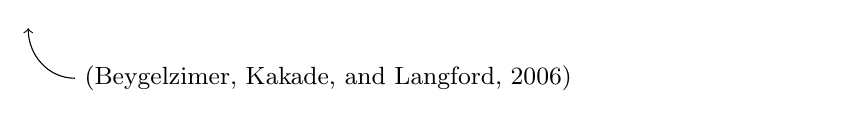
\begin{tikzpicture}
%\node (a) {\small (Beygelzimer \emph{et. al.}, 2006)};
\node (a) {\small (Beygelzimer, Kakade, and Langford, 2006)};
\node at (2.5in,0) {};
\draw[->] (a) to[out=180,in=270]  (-1.5in,0.25in);
\end{tikzpicture}
\end{center}
\end{frame}

%%%%%%%%%%%%%%%%%%%%%%%%%%%%%%%%%%%%%%%%%%%%%%%%%%%%%%%%%%%%%%%%%%%%%%%%%%%%%%%%

\begin{frame}{Other uses of cover trees}

\Large
Any learning algorithm that cares about distance can be made faster using cover trees.
\vspace{0.15in}

Examples:
\begin{itemize}
\item $k$-nearest neighbor
\item Support vector machines (Segata and Blanzieri, 2010)
\item Dimensionality reduction (Lisitsyn \emph{et. al.}, 2010)
%\item Clustering
\item Reinforcement learning (Tziortziotis \emph{et. al.}, 2014)
\end{itemize}

\end{frame}


%%%%%%%%%%%%%%%%%%%%%%%%%%%%%%%%%%%%%%%

\begin{frame}[fragile]{Outline}
\LARGE
\centering
\begin{itemize}
\item
Why care about faster cover trees?
\vspace{0.2in}
\item
Making cover trees faster.
\begin{itemize}
\Large
\vspace{0.1in}
\item Experimental setup
\vspace{0.1in}
\item Simpler definition reduces the number of nodes
\vspace{0.1in}
\item The nearest ancestor invariant
\vspace{0.1in}
\item Better cache performance
\vspace{0.1in}
\item Constructing and querying the tree in parallel
\end{itemize}
\end{itemize}
\end{frame}

%%%%%%%%%%%%%%%%%%%%%%%%%%%%%%%%%%%%%%%

\begin{frame}{Experimental setup}
\Large

Three data sources:
\begin{itemize}
\item MLPack benchmarks with Euclidean distance
    %\begin{itemize}
    %\item Selected the 8 largest datasets
    %\item Maximum size
    %\end{itemize}
\item Protein dataset with the random walk graph distance
\item Yahoo! 1.5 million creative common images with the earth movers distance
\end{itemize}

\vspace{0.15in}
Benchmarking procedure:
\begin{itemize}
\item Construct a cover tree on the dataset
\item For each data point in the dataset, find the nearest neighbor
\end{itemize}

\end{frame}

\begin{frame}[fragile]{The simplified cover tree}

\begin{center}
\begin{tikzpicture}
    [ draw
    , every node/.style={minimum size=10mm,fill=white}
    , level/.style={sibling distance = 23mm/#1, level distance=12mm}
    %,    level distance = 1.5cm}
    , sibling distance=8mm
    ]
\draw (-2.3,0) -- (8.6,0)[dotted];
\draw (-2.3,-12mm) -- (8.6,-12mm)[dotted];
\draw (-2.3,-24mm) -- (8.6,-24mm)[dotted];
\node[shape=circle,draw] at (2.5,0) {10}
    child { node[circle,draw] {8}
        child { node[circle,draw] {7}  }
        child { node[circle,draw] {9} }
        }
    child { node[circle,draw] {12}
        %child { node[circle,draw,fill=lightred,line width=1pt] {9}  }
        %child { node[circle,draw] {13} }
        }
    ;
%\node[shape=circle,draw] at (5,0) {10}
    %child { node[circle,draw] {8}
        %child { node[circle,draw] {7}  }
        %child { node[circle,draw,fill=lightgreen,line width=1pt] {9} }
        %}
    %child { node[circle,draw] {12}
        %child { node[circle,draw,fill=lightgreen,line width=1pt] {11}  }
        %child { node[circle,draw] {13} }
        %}
    %;
\node[fill=none] at (8,3mm) {level 3};
\node[fill=none] at (8,-9mm) {level 2};
\node[fill=none] at (8,-21mm) {level 1};
\end{tikzpicture}
\end{center}

\uncover<1> {
%\vspace{0.15in}
\textbf{The covering invariant.}
For every node $p$, define the function $\covdist p = \exprad p^{\level p}$.
For each child $q$ of $p$
$$
\dist p q \le \covdist p
$$

\vspace{0.15in}
\textbf{The separating invariant.}
For every node $p$, define the function $\sepdist p = \exprad p^{\level p-1}$.
For all distinct children $q_1$ and $q_2$ of $p$
$$
\dist{q_1}{q_2} \ge \sepdist p
$$
}

\uncover<2> {
\vspace{-1.70in}
Advantages of the simplified cover tree:
\vspace{0.05in}
\begin{itemize}
\item Maintains all runtime guarantees of the original cover tree.
\vspace{0.05in}

\item Significantly easier to understand and implement.

%\vspace{0.05in}
The original cover tree was described in terms of an infinitely large tree, only a subset of which actually gets implemented.

\vspace{0.05in}
\item Requires exactly $n$ nodes instead of $O(n)$ nodes.

%\vspace{0.05in}
Fewer nodes means a faster constant factor for all algorithms. %insertions and queries are faster.
\end{itemize}
\vspace{1.3in}
}

\end{frame}


\begin{frame}[fragile]{The simplified cover tree}

\centering
\graphicspath{{slides/paperimg/}}
% GNUPLOT: LaTeX picture with Postscript
\begingroup
  \makeatletter
  \providecommand\color[2][]{%
    \GenericError{(gnuplot) \space\space\space\@spaces}{%
      Package color not loaded in conjunction with
      terminal option `colourtext'%
    }{See the gnuplot documentation for explanation.%
    }{Either use 'blacktext' in gnuplot or load the package
      color.sty in LaTeX.}%
    \renewcommand\color[2][]{}%
  }%
  \providecommand\includegraphics[2][]{%
    \GenericError{(gnuplot) \space\space\space\@spaces}{%
      Package graphicx or graphics not loaded%
    }{See the gnuplot documentation for explanation.%
    }{The gnuplot epslatex terminal needs graphicx.sty or graphics.sty.}%
    \renewcommand\includegraphics[2][]{}%
  }%
  \providecommand\rotatebox[2]{#2}%
  \@ifundefined{ifGPcolor}{%
    \newif\ifGPcolor
    \GPcolortrue
  }{}%
  \@ifundefined{ifGPblacktext}{%
    \newif\ifGPblacktext
    \GPblacktextfalse
  }{}%
  % define a \g@addto@macro without @ in the name:
  \let\gplgaddtomacro\g@addto@macro
  % define empty templates for all commands taking text:
  \gdef\gplbacktext{}%
  \gdef\gplfronttext{}%
  \makeatother
  \ifGPblacktext
    % no textcolor at all
    \def\colorrgb#1{}%
    \def\colorgray#1{}%
  \else
    % gray or color?
    \ifGPcolor
      \def\colorrgb#1{\color[rgb]{#1}}%
      \def\colorgray#1{\color[gray]{#1}}%
      \expandafter\def\csname LTw\endcsname{\color{white}}%
      \expandafter\def\csname LTb\endcsname{\color{black}}%
      \expandafter\def\csname LTa\endcsname{\color{black}}%
      \expandafter\def\csname LT0\endcsname{\color[rgb]{1,0,0}}%
      \expandafter\def\csname LT1\endcsname{\color[rgb]{0,1,0}}%
      \expandafter\def\csname LT2\endcsname{\color[rgb]{0,0,1}}%
      \expandafter\def\csname LT3\endcsname{\color[rgb]{1,0,1}}%
      \expandafter\def\csname LT4\endcsname{\color[rgb]{0,1,1}}%
      \expandafter\def\csname LT5\endcsname{\color[rgb]{1,1,0}}%
      \expandafter\def\csname LT6\endcsname{\color[rgb]{0,0,0}}%
      \expandafter\def\csname LT7\endcsname{\color[rgb]{1,0.3,0}}%
      \expandafter\def\csname LT8\endcsname{\color[rgb]{0.5,0.5,0.5}}%
    \else
      % gray
      \def\colorrgb#1{\color{black}}%
      \def\colorgray#1{\color[gray]{#1}}%
      \expandafter\def\csname LTw\endcsname{\color{white}}%
      \expandafter\def\csname LTb\endcsname{\color{black}}%
      \expandafter\def\csname LTa\endcsname{\color{black}}%
      \expandafter\def\csname LT0\endcsname{\color{black}}%
      \expandafter\def\csname LT1\endcsname{\color{black}}%
      \expandafter\def\csname LT2\endcsname{\color{black}}%
      \expandafter\def\csname LT3\endcsname{\color{black}}%
      \expandafter\def\csname LT4\endcsname{\color{black}}%
      \expandafter\def\csname LT5\endcsname{\color{black}}%
      \expandafter\def\csname LT6\endcsname{\color{black}}%
      \expandafter\def\csname LT7\endcsname{\color{black}}%
      \expandafter\def\csname LT8\endcsname{\color{black}}%
    \fi
  \fi
  \setlength{\unitlength}{0.0500bp}%
  \begin{picture}(5040.00,3772.00)%
    \gplgaddtomacro\gplbacktext{%
      \csname LTb\endcsname%
      \put(1166,780){\makebox(0,0)[r]{\strut{} 0}}%
      \put(1166,1053){\makebox(0,0)[r]{\strut{} 0.1}}%
      \put(1166,1325){\makebox(0,0)[r]{\strut{} 0.2}}%
      \put(1166,1598){\makebox(0,0)[r]{\strut{} 0.3}}%
      \put(1166,1871){\makebox(0,0)[r]{\strut{} 0.4}}%
      \put(1166,2144){\makebox(0,0)[r]{\strut{} 0.5}}%
      \put(1166,2416){\makebox(0,0)[r]{\strut{} 0.6}}%
      \put(1166,2689){\makebox(0,0)[r]{\strut{} 0.7}}%
      \put(1166,2962){\makebox(0,0)[r]{\strut{} 0.8}}%
      \put(1166,3234){\makebox(0,0)[r]{\strut{} 0.9}}%
      \put(1166,3507){\makebox(0,0)[r]{\strut{} 1}}%
      \put(1661,648){\rotatebox{-45}{\makebox(0,0)[l]{\strut{}yearpredict}}}%
      \put(2023,648){\rotatebox{-45}{\makebox(0,0)[l]{\strut{}twitter}}}%
      \put(2386,648){\rotatebox{-45}{\makebox(0,0)[l]{\strut{}tinyImages}}}%
      \put(2748,648){\rotatebox{-45}{\makebox(0,0)[l]{\strut{}mnist}}}%
      \put(3111,648){\rotatebox{-45}{\makebox(0,0)[l]{\strut{}corel}}}%
      \put(3473,648){\rotatebox{-45}{\makebox(0,0)[l]{\strut{}covtype}}}%
      \put(3836,648){\rotatebox{-45}{\makebox(0,0)[l]{\strut{}artificial40}}}%
      \put(4198,648){\rotatebox{-45}{\makebox(0,0)[l]{\strut{}faces}}}%
      \put(176,2143){\rotatebox{-270}{\makebox(0,0){\strut{}fraction of nodes in the original cover tree }}}%
      \put(396,2143){\rotatebox{-270}{\makebox(0,0){\strut{} required for the simplified cover tree}}}%
    }%
    \gplgaddtomacro\gplfronttext{%
    }%
    \gplbacktext
    \put(0,0){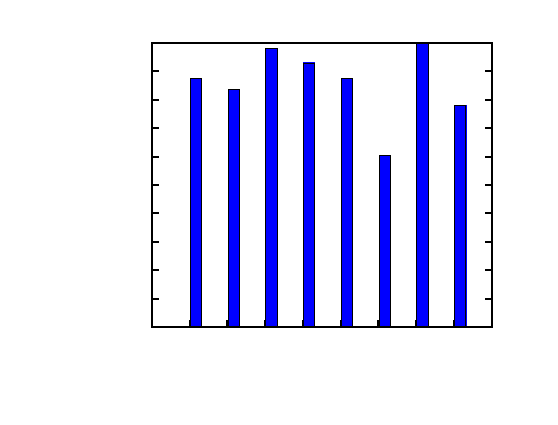
\includegraphics{nodes}}%
    \gplfronttext
  \end{picture}%
\endgroup


\end{frame}

\begin{frame}[fragile]{The nearest ancestor cover tree}

\definecolor{lightred}{rgb}{1,0.8,0.8}
\definecolor{lightgreen}{rgb}{0.8,1,0.8}
\begin{center}
\begin{tikzpicture}
    [ draw
    , every node/.style={minimum size=10mm,fill=white}
    , level/.style={sibling distance = 23mm/#1, level distance=12mm}
    %,    level distance = 1.5cm}
    , sibling distance=8mm
    ]
\draw (-2.3,0) -- (8.6,0)[dotted];
\draw (-2.3,-12mm) -- (8.6,-12mm)[dotted];
\draw (-2.3,-24mm) -- (8.6,-24mm)[dotted];
\node[shape=circle,draw] at (0,0) {10}
    child { node[circle,draw] {8}
        child { node[circle,draw] {7}  }
        child { node[circle,draw,fill=lightred,line width=1pt] {11} }
        }
    child { node[circle,draw] {12}
        child { node[circle,draw,fill=lightred,line width=1pt] {9}  }
        child { node[circle,draw] {13} }
        }
    ;
\node[shape=circle,draw] at (5,0) {10}
    child { node[circle,draw] {8}
        child { node[circle,draw] {7}  }
        child { node[circle,draw,fill=lightgreen,line width=1pt] {9} }
        }
    child { node[circle,draw] {12}
        child { node[circle,draw,fill=lightgreen,line width=1pt] {11}  }
        child { node[circle,draw] {13} }
        }
    ;
\node[fill=none] at (8,3mm) {level 3};
\node[fill=none] at (8,-9mm) {level 2};
\node[fill=none] at (8,-21mm) {level 1};
\end{tikzpicture}
\end{center}

\uncover<1> {
A \textbf{nearest ancestor cover tree} is a simplified cover tree where every point $p$ satisfies the additional invariant that if $q_1$ is an ancestor of $p$ and $q_2$ is a sibling of $q_1$, then
$$
d(p,q_1) \le d(p,q_2)
$$
}

%\vspace{0.15in}
%Insertion requires rebalancing.
\uncover<2> {
\vspace{-1.1in}
Insertions require rebalancing.

\vspace{0.15in}
No runtime guarantees on the rebalance step.

\vspace{0.15in}
In practice, queries are much faster and construction is only slightly slower.
}
\end{frame}

%%%%%%%%%%%%%%%%%%%%%%%%%%%%%%%%%%%%%%%%%%%%%%%%%%%%%%%%%%%%%%%%%%%%%%%%%%%%%%%%

\begin{frame}[fragile]{Comparing cover trees on \emph{construction} time}
\centering
\graphicspath{{covertree/paperimg/}}
% GNUPLOT: LaTeX picture with Postscript
\begingroup
  \makeatletter
  \providecommand\color[2][]{%
    \GenericError{(gnuplot) \space\space\space\@spaces}{%
      Package color not loaded in conjunction with
      terminal option `colourtext'%
    }{See the gnuplot documentation for explanation.%
    }{Either use 'blacktext' in gnuplot or load the package
      color.sty in LaTeX.}%
    \renewcommand\color[2][]{}%
  }%
  \providecommand\includegraphics[2][]{%
    \GenericError{(gnuplot) \space\space\space\@spaces}{%
      Package graphicx or graphics not loaded%
    }{See the gnuplot documentation for explanation.%
    }{The gnuplot epslatex terminal needs graphicx.sty or graphics.sty.}%
    \renewcommand\includegraphics[2][]{}%
  }%
  \providecommand\rotatebox[2]{#2}%
  \@ifundefined{ifGPcolor}{%
    \newif\ifGPcolor
    \GPcolortrue
  }{}%
  \@ifundefined{ifGPblacktext}{%
    \newif\ifGPblacktext
    \GPblacktextfalse
  }{}%
  % define a \g@addto@macro without @ in the name:
  \let\gplgaddtomacro\g@addto@macro
  % define empty templates for all commands taking text:
  \gdef\gplbacktext{}%
  \gdef\gplfronttext{}%
  \makeatother
  \ifGPblacktext
    % no textcolor at all
    \def\colorrgb#1{}%
    \def\colorgray#1{}%
  \else
    % gray or color?
    \ifGPcolor
      \def\colorrgb#1{\color[rgb]{#1}}%
      \def\colorgray#1{\color[gray]{#1}}%
      \expandafter\def\csname LTw\endcsname{\color{white}}%
      \expandafter\def\csname LTb\endcsname{\color{black}}%
      \expandafter\def\csname LTa\endcsname{\color{black}}%
      \expandafter\def\csname LT0\endcsname{\color[rgb]{1,0,0}}%
      \expandafter\def\csname LT1\endcsname{\color[rgb]{0,1,0}}%
      \expandafter\def\csname LT2\endcsname{\color[rgb]{0,0,1}}%
      \expandafter\def\csname LT3\endcsname{\color[rgb]{1,0,1}}%
      \expandafter\def\csname LT4\endcsname{\color[rgb]{0,1,1}}%
      \expandafter\def\csname LT5\endcsname{\color[rgb]{1,1,0}}%
      \expandafter\def\csname LT6\endcsname{\color[rgb]{0,0,0}}%
      \expandafter\def\csname LT7\endcsname{\color[rgb]{1,0.3,0}}%
      \expandafter\def\csname LT8\endcsname{\color[rgb]{0.5,0.5,0.5}}%
    \else
      % gray
      \def\colorrgb#1{\color{black}}%
      \def\colorgray#1{\color[gray]{#1}}%
      \expandafter\def\csname LTw\endcsname{\color{white}}%
      \expandafter\def\csname LTb\endcsname{\color{black}}%
      \expandafter\def\csname LTa\endcsname{\color{black}}%
      \expandafter\def\csname LT0\endcsname{\color{black}}%
      \expandafter\def\csname LT1\endcsname{\color{black}}%
      \expandafter\def\csname LT2\endcsname{\color{black}}%
      \expandafter\def\csname LT3\endcsname{\color{black}}%
      \expandafter\def\csname LT4\endcsname{\color{black}}%
      \expandafter\def\csname LT5\endcsname{\color{black}}%
      \expandafter\def\csname LT6\endcsname{\color{black}}%
      \expandafter\def\csname LT7\endcsname{\color{black}}%
      \expandafter\def\csname LT8\endcsname{\color{black}}%
    \fi
  \fi
  \setlength{\unitlength}{0.0500bp}%
  \begin{picture}(5040.00,3772.00)%
    \gplgaddtomacro\gplbacktext{%
      \csname LTb\endcsname%
      \put(1122,780){\makebox(0,0)[r]{\strut{} 0}}%
      \put(1122,1235){\makebox(0,0)[r]{\strut{} 1}}%
      \put(1122,1689){\makebox(0,0)[r]{\strut{} 2}}%
      \put(1122,2144){\makebox(0,0)[r]{\strut{} 3}}%
      \put(1122,2598){\makebox(0,0)[r]{\strut{} 4}}%
      \put(1122,3053){\makebox(0,0)[r]{\strut{} 5}}%
      \put(1622,648){\rotatebox{-45}{\makebox(0,0)[l]{\strut{}yearpredict}}}%
      \put(1991,648){\rotatebox{-45}{\makebox(0,0)[l]{\strut{}twitter}}}%
      \put(2359,648){\rotatebox{-45}{\makebox(0,0)[l]{\strut{}tinyImages}}}%
      \put(2728,648){\rotatebox{-45}{\makebox(0,0)[l]{\strut{}mnist}}}%
      \put(3096,648){\rotatebox{-45}{\makebox(0,0)[l]{\strut{}corel}}}%
      \put(3465,648){\rotatebox{-45}{\makebox(0,0)[l]{\strut{}covtype}}}%
      \put(3833,648){\rotatebox{-45}{\makebox(0,0)[l]{\strut{}artificial40}}}%
      \put(4202,648){\rotatebox{-45}{\makebox(0,0)[l]{\strut{}faces}}}%
      \put(176,2143){\rotatebox{-270}{\makebox(0,0){\strut{}number of distance comparisons}}}%
      \put(396,2143){\rotatebox{-270}{\makebox(0,0){\strut{}in tree \emph{construction} only}}}%
      \put(616,2143){\rotatebox{-270}{\makebox(0,0){\strut{}(normalized by the original cover tree)}}}%
      \put(2016,3205){\makebox(0,0)[l]{\strut{}19.1}}%
    }%
    \gplgaddtomacro\gplfronttext{%
    }%
    \gplbacktext
    \put(0,0){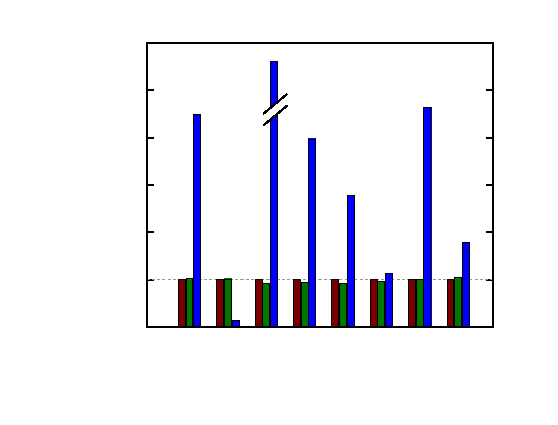
\includegraphics{numdist_insert}}%
    \gplfronttext
  \end{picture}%
\endgroup

\begin{tikzpicture}
    \node[draw,fill=darkred,minimum width=0.03in,minimum height=0.3in] at (0,0) {};
    \node at (0,0.77in) {\small\rotatebox{90}{Original cover tree}};
    \node[draw,fill=darkgreen,minimum width=0.03in,minimum height=0.3in] at (0.15in,0) {};
    \node at (0.15in,0.82in) {\small\rotatebox{90}{Simplified cover tree}};
    \node[draw,fill=blue,minimum width=0.03in,minimum height=0.3in] at (0.3in,0) {};
    \node at (0.3in,1.01in) {\small\rotatebox{90}{Nearest ancestor cover tree}};
    \node[minimum width=0.05in,minimum height=0.5in] at (0.45in,0) {};
    \node at (0.45in,0.6in) {\small\rotatebox{90}{}};
    \node at (0,-0.5in) {};
\end{tikzpicture}
\end{frame}

%%%%%%%%%%%%%%%%%%%%%%%%%%%%%%%%%%%%%%%%%%%%%%%%%%%%%%%%%%%%%%%%%%%%%%%%%%%%%%%%

\begin{frame}[fragile]{Comparing cover trees on \emph{construction and query} time}
\centering
\graphicspath{{covertree/paperimg/}}
% GNUPLOT: LaTeX picture with Postscript
\begingroup
  \makeatletter
  \providecommand\color[2][]{%
    \GenericError{(gnuplot) \space\space\space\@spaces}{%
      Package color not loaded in conjunction with
      terminal option `colourtext'%
    }{See the gnuplot documentation for explanation.%
    }{Either use 'blacktext' in gnuplot or load the package
      color.sty in LaTeX.}%
    \renewcommand\color[2][]{}%
  }%
  \providecommand\includegraphics[2][]{%
    \GenericError{(gnuplot) \space\space\space\@spaces}{%
      Package graphicx or graphics not loaded%
    }{See the gnuplot documentation for explanation.%
    }{The gnuplot epslatex terminal needs graphicx.sty or graphics.sty.}%
    \renewcommand\includegraphics[2][]{}%
  }%
  \providecommand\rotatebox[2]{#2}%
  \@ifundefined{ifGPcolor}{%
    \newif\ifGPcolor
    \GPcolortrue
  }{}%
  \@ifundefined{ifGPblacktext}{%
    \newif\ifGPblacktext
    \GPblacktextfalse
  }{}%
  % define a \g@addto@macro without @ in the name:
  \let\gplgaddtomacro\g@addto@macro
  % define empty templates for all commands taking text:
  \gdef\gplbacktext{}%
  \gdef\gplfronttext{}%
  \makeatother
  \ifGPblacktext
    % no textcolor at all
    \def\colorrgb#1{}%
    \def\colorgray#1{}%
  \else
    % gray or color?
    \ifGPcolor
      \def\colorrgb#1{\color[rgb]{#1}}%
      \def\colorgray#1{\color[gray]{#1}}%
      \expandafter\def\csname LTw\endcsname{\color{white}}%
      \expandafter\def\csname LTb\endcsname{\color{black}}%
      \expandafter\def\csname LTa\endcsname{\color{black}}%
      \expandafter\def\csname LT0\endcsname{\color[rgb]{1,0,0}}%
      \expandafter\def\csname LT1\endcsname{\color[rgb]{0,1,0}}%
      \expandafter\def\csname LT2\endcsname{\color[rgb]{0,0,1}}%
      \expandafter\def\csname LT3\endcsname{\color[rgb]{1,0,1}}%
      \expandafter\def\csname LT4\endcsname{\color[rgb]{0,1,1}}%
      \expandafter\def\csname LT5\endcsname{\color[rgb]{1,1,0}}%
      \expandafter\def\csname LT6\endcsname{\color[rgb]{0,0,0}}%
      \expandafter\def\csname LT7\endcsname{\color[rgb]{1,0.3,0}}%
      \expandafter\def\csname LT8\endcsname{\color[rgb]{0.5,0.5,0.5}}%
    \else
      % gray
      \def\colorrgb#1{\color{black}}%
      \def\colorgray#1{\color[gray]{#1}}%
      \expandafter\def\csname LTw\endcsname{\color{white}}%
      \expandafter\def\csname LTb\endcsname{\color{black}}%
      \expandafter\def\csname LTa\endcsname{\color{black}}%
      \expandafter\def\csname LT0\endcsname{\color{black}}%
      \expandafter\def\csname LT1\endcsname{\color{black}}%
      \expandafter\def\csname LT2\endcsname{\color{black}}%
      \expandafter\def\csname LT3\endcsname{\color{black}}%
      \expandafter\def\csname LT4\endcsname{\color{black}}%
      \expandafter\def\csname LT5\endcsname{\color{black}}%
      \expandafter\def\csname LT6\endcsname{\color{black}}%
      \expandafter\def\csname LT7\endcsname{\color{black}}%
      \expandafter\def\csname LT8\endcsname{\color{black}}%
    \fi
  \fi
  \setlength{\unitlength}{0.0500bp}%
  \begin{picture}(5040.00,3772.00)%
    \gplgaddtomacro\gplbacktext{%
      \csname LTb\endcsname%
      \put(1122,780){\makebox(0,0)[r]{\strut{} 0}}%
      \put(1122,1235){\makebox(0,0)[r]{\strut{} 0.2}}%
      \put(1122,1689){\makebox(0,0)[r]{\strut{} 0.4}}%
      \put(1122,2144){\makebox(0,0)[r]{\strut{} 0.6}}%
      \put(1122,2598){\makebox(0,0)[r]{\strut{} 0.8}}%
      \put(1122,3052){\makebox(0,0)[r]{\strut{} 1}}%
      \put(1122,3507){\makebox(0,0)[r]{\strut{} 1.2}}%
      \put(1622,648){\rotatebox{-45}{\makebox(0,0)[l]{\strut{}yearpredict}}}%
      \put(1991,648){\rotatebox{-45}{\makebox(0,0)[l]{\strut{}twitter}}}%
      \put(2359,648){\rotatebox{-45}{\makebox(0,0)[l]{\strut{}tinyImages}}}%
      \put(2728,648){\rotatebox{-45}{\makebox(0,0)[l]{\strut{}mnist}}}%
      \put(3096,648){\rotatebox{-45}{\makebox(0,0)[l]{\strut{}corel}}}%
      \put(3465,648){\rotatebox{-45}{\makebox(0,0)[l]{\strut{}covtype}}}%
      \put(3833,648){\rotatebox{-45}{\makebox(0,0)[l]{\strut{}artificial40}}}%
      \put(4202,648){\rotatebox{-45}{\makebox(0,0)[l]{\strut{}faces}}}%
      \put(176,2143){\rotatebox{-270}{\makebox(0,0){\strut{}number of distance comparisons}}}%
      \put(396,2143){\rotatebox{-270}{\makebox(0,0){\strut{}in tree \emph{construction} and \emph{query}}}}%
      \put(616,2143){\rotatebox{-270}{\makebox(0,0){\strut{}(normalized by $n^2$)}}}%
    }%
    \gplgaddtomacro\gplfronttext{%
    }%
    \gplbacktext
    \put(0,0){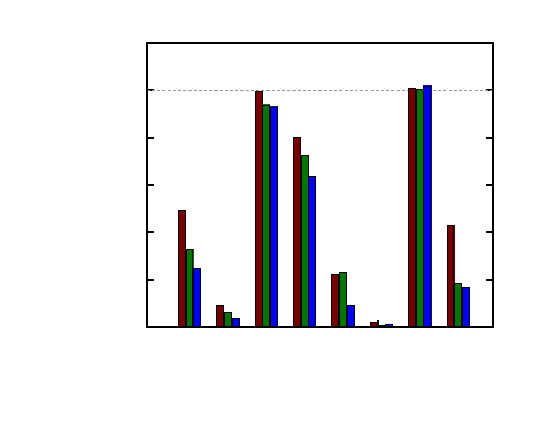
\includegraphics{numdist}}%
    \gplfronttext
  \end{picture}%
\endgroup

\begin{tikzpicture}
    \node[draw,fill=darkred,minimum width=0.03in,minimum height=0.3in] at (0,0) {};
    \node at (0,0.77in) {\small\rotatebox{90}{Original cover tree}};
    \node[draw,fill=darkgreen,minimum width=0.03in,minimum height=0.3in] at (0.15in,0) {};
    \node at (0.15in,0.82in) {\small\rotatebox{90}{Simplified cover tree}};
    \node[draw,fill=blue,minimum width=0.03in,minimum height=0.3in] at (0.3in,0) {};
    \node at (0.3in,1.01in) {\small\rotatebox{90}{Nearest ancestor cover tree}};
    \node[minimum width=0.05in,minimum height=0.5in] at (0.45in,0) {};
    \node at (0.45in,0.6in) {\small\rotatebox{90}{}};
    \node at (0,-0.5in) {};
\end{tikzpicture}
\end{frame}

%%%%%%%%%%%%%%%%%%%%%%%%%%%%%%%%%%%%%%%%%%%%%%%%%%%%%%%%%%%%%%%%%%%%%%%%%%%%%%%%

\begin{frame}[fragile]{All of the cover trees scale similarly}

This experiment uses the protein data and the random walk graph kernel.
\vspace{0.15in}

{
\centering
\graphicspath{{covertree/paperimg/}}
% GNUPLOT: LaTeX picture with Postscript
\begingroup
  \makeatletter
  \providecommand\color[2][]{%
    \GenericError{(gnuplot) \space\space\space\@spaces}{%
      Package color not loaded in conjunction with
      terminal option `colourtext'%
    }{See the gnuplot documentation for explanation.%
    }{Either use 'blacktext' in gnuplot or load the package
      color.sty in LaTeX.}%
    \renewcommand\color[2][]{}%
  }%
  \providecommand\includegraphics[2][]{%
    \GenericError{(gnuplot) \space\space\space\@spaces}{%
      Package graphicx or graphics not loaded%
    }{See the gnuplot documentation for explanation.%
    }{The gnuplot epslatex terminal needs graphicx.sty or graphics.sty.}%
    \renewcommand\includegraphics[2][]{}%
  }%
  \providecommand\rotatebox[2]{#2}%
  \@ifundefined{ifGPcolor}{%
    \newif\ifGPcolor
    \GPcolortrue
  }{}%
  \@ifundefined{ifGPblacktext}{%
    \newif\ifGPblacktext
    \GPblacktextfalse
  }{}%
  % define a \g@addto@macro without @ in the name:
  \let\gplgaddtomacro\g@addto@macro
  % define empty templates for all commands taking text:
  \gdef\gplbacktext{}%
  \gdef\gplfronttext{}%
  \makeatother
  \ifGPblacktext
    % no textcolor at all
    \def\colorrgb#1{}%
    \def\colorgray#1{}%
  \else
    % gray or color?
    \ifGPcolor
      \def\colorrgb#1{\color[rgb]{#1}}%
      \def\colorgray#1{\color[gray]{#1}}%
      \expandafter\def\csname LTw\endcsname{\color{white}}%
      \expandafter\def\csname LTb\endcsname{\color{black}}%
      \expandafter\def\csname LTa\endcsname{\color{black}}%
      \expandafter\def\csname LT0\endcsname{\color[rgb]{1,0,0}}%
      \expandafter\def\csname LT1\endcsname{\color[rgb]{0,1,0}}%
      \expandafter\def\csname LT2\endcsname{\color[rgb]{0,0,1}}%
      \expandafter\def\csname LT3\endcsname{\color[rgb]{1,0,1}}%
      \expandafter\def\csname LT4\endcsname{\color[rgb]{0,1,1}}%
      \expandafter\def\csname LT5\endcsname{\color[rgb]{1,1,0}}%
      \expandafter\def\csname LT6\endcsname{\color[rgb]{0,0,0}}%
      \expandafter\def\csname LT7\endcsname{\color[rgb]{1,0.3,0}}%
      \expandafter\def\csname LT8\endcsname{\color[rgb]{0.5,0.5,0.5}}%
    \else
      % gray
      \def\colorrgb#1{\color{black}}%
      \def\colorgray#1{\color[gray]{#1}}%
      \expandafter\def\csname LTw\endcsname{\color{white}}%
      \expandafter\def\csname LTb\endcsname{\color{black}}%
      \expandafter\def\csname LTa\endcsname{\color{black}}%
      \expandafter\def\csname LT0\endcsname{\color{black}}%
      \expandafter\def\csname LT1\endcsname{\color{black}}%
      \expandafter\def\csname LT2\endcsname{\color{black}}%
      \expandafter\def\csname LT3\endcsname{\color{black}}%
      \expandafter\def\csname LT4\endcsname{\color{black}}%
      \expandafter\def\csname LT5\endcsname{\color{black}}%
      \expandafter\def\csname LT6\endcsname{\color{black}}%
      \expandafter\def\csname LT7\endcsname{\color{black}}%
      \expandafter\def\csname LT8\endcsname{\color{black}}%
    \fi
  \fi
  \setlength{\unitlength}{0.0500bp}%
  \begin{picture}(5040.00,3772.00)%
    \gplgaddtomacro\gplbacktext{%
      \csname LTb\endcsname%
      \put(1298,704){\makebox(0,0)[r]{\strut{} 0}}%
      \put(1298,1054){\makebox(0,0)[r]{\strut{} 200}}%
      \put(1298,1405){\makebox(0,0)[r]{\strut{} 400}}%
      \put(1298,1755){\makebox(0,0)[r]{\strut{} 600}}%
      \put(1298,2106){\makebox(0,0)[r]{\strut{} 800}}%
      \put(1298,2456){\makebox(0,0)[r]{\strut{} 1000}}%
      \put(1298,2806){\makebox(0,0)[r]{\strut{} 1200}}%
      \put(1298,3157){\makebox(0,0)[r]{\strut{} 1400}}%
      \put(1298,3507){\makebox(0,0)[r]{\strut{} 1600}}%
      \put(1430,484){\makebox(0,0){\strut{} 0}}%
      \put(2073,484){\makebox(0,0){\strut{} 50}}%
      \put(2715,484){\makebox(0,0){\strut{} 100}}%
      \put(3358,484){\makebox(0,0){\strut{} 150}}%
      \put(4000,484){\makebox(0,0){\strut{} 200}}%
      \put(4643,484){\makebox(0,0){\strut{} 250}}%
      \put(176,2105){\rotatebox{-270}{\makebox(0,0){\strut{}total distance comparisons (millions)}}}%
      \put(396,2105){\rotatebox{-270}{\makebox(0,0){\strut{}on \emph{construction} and \emph{query}}}}%
      \put(3036,154){\makebox(0,0){\strut{}number of data points (thousands)}}%
    }%
    \gplgaddtomacro\gplfronttext{%
    }%
    \gplbacktext
    \put(0,0){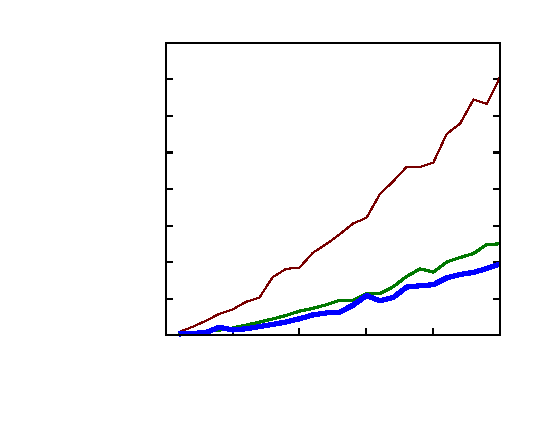
\includegraphics{protein-simple}}%
    \gplfronttext
  \end{picture}%
\endgroup

\begin{tikzpicture}
    \node[draw,fill=darkred,minimum width=0.03in,minimum height=0.3in] at (0,0) {};
    \node at (0,0.77in) {\small\rotatebox{90}{Original cover tree}};
    \node[draw,fill=darkgreen,minimum width=0.03in,minimum height=0.3in] at (0.15in,0) {};
    \node at (0.15in,0.82in) {\small\rotatebox{90}{Simplified cover tree}};
    \node[draw,fill=blue,minimum width=0.03in,minimum height=0.3in] at (0.3in,0) {};
    \node at (0.3in,1.01in) {\small\rotatebox{90}{Nearest ancestor cover tree}};
    \node[minimum width=0.05in,minimum height=0.5in] at (0.45in,0) {};
    %\node at (0.6in,0.7in) {\small\rotatebox{90}{ dotted lines: construction only}};
    %\node at (0.75in,0.81in) {\small\rotatebox{90}{ solid lines: construction and query}};
    \node at (0,-0.5in) {};
\end{tikzpicture}
}

\end{frame}

\begin{frame}[fragile]{Cache oblivious cover tree}

%RAM model is a lie
%
%\vspace{0.1in}
Need to consider cache accesses for fast, modern data structures

%\vspace{0.1in}
%In a \emph{cache oblivious} data structure, the programmer doesn't need to know any details about the underlying hardware
%
\begin{center}
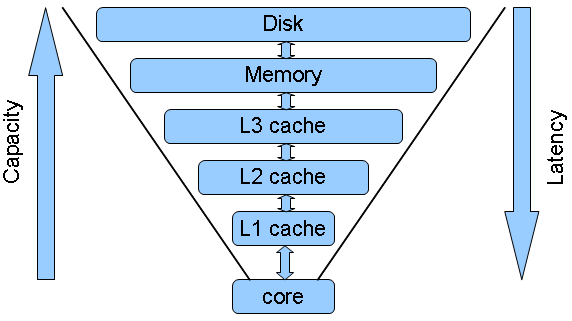
\includegraphics[width=10cm]{slides/cpu_cache_structure}
\end{center}

{\tiny image from: \url{http://1024cores.net} }
\end{frame}

%%%%%%%%%%%%%%%%%%%%%%%%%%%%%%%%%%%%%%%%%%%%%%%%%%%%%%%%%%%%%%%%%%%%%%%%%%%%%%%%

\begin{frame}[fragile]{Cache oblivious cover tree}

%The trick: use the van Emde Boas tree layout
Arrange nodes in memory according to a preorder traversal of the tree

(van Emde Boas \emph{et al.}, 1966; Demaine, 2002)
\vspace{0.1in}

\begin{center}
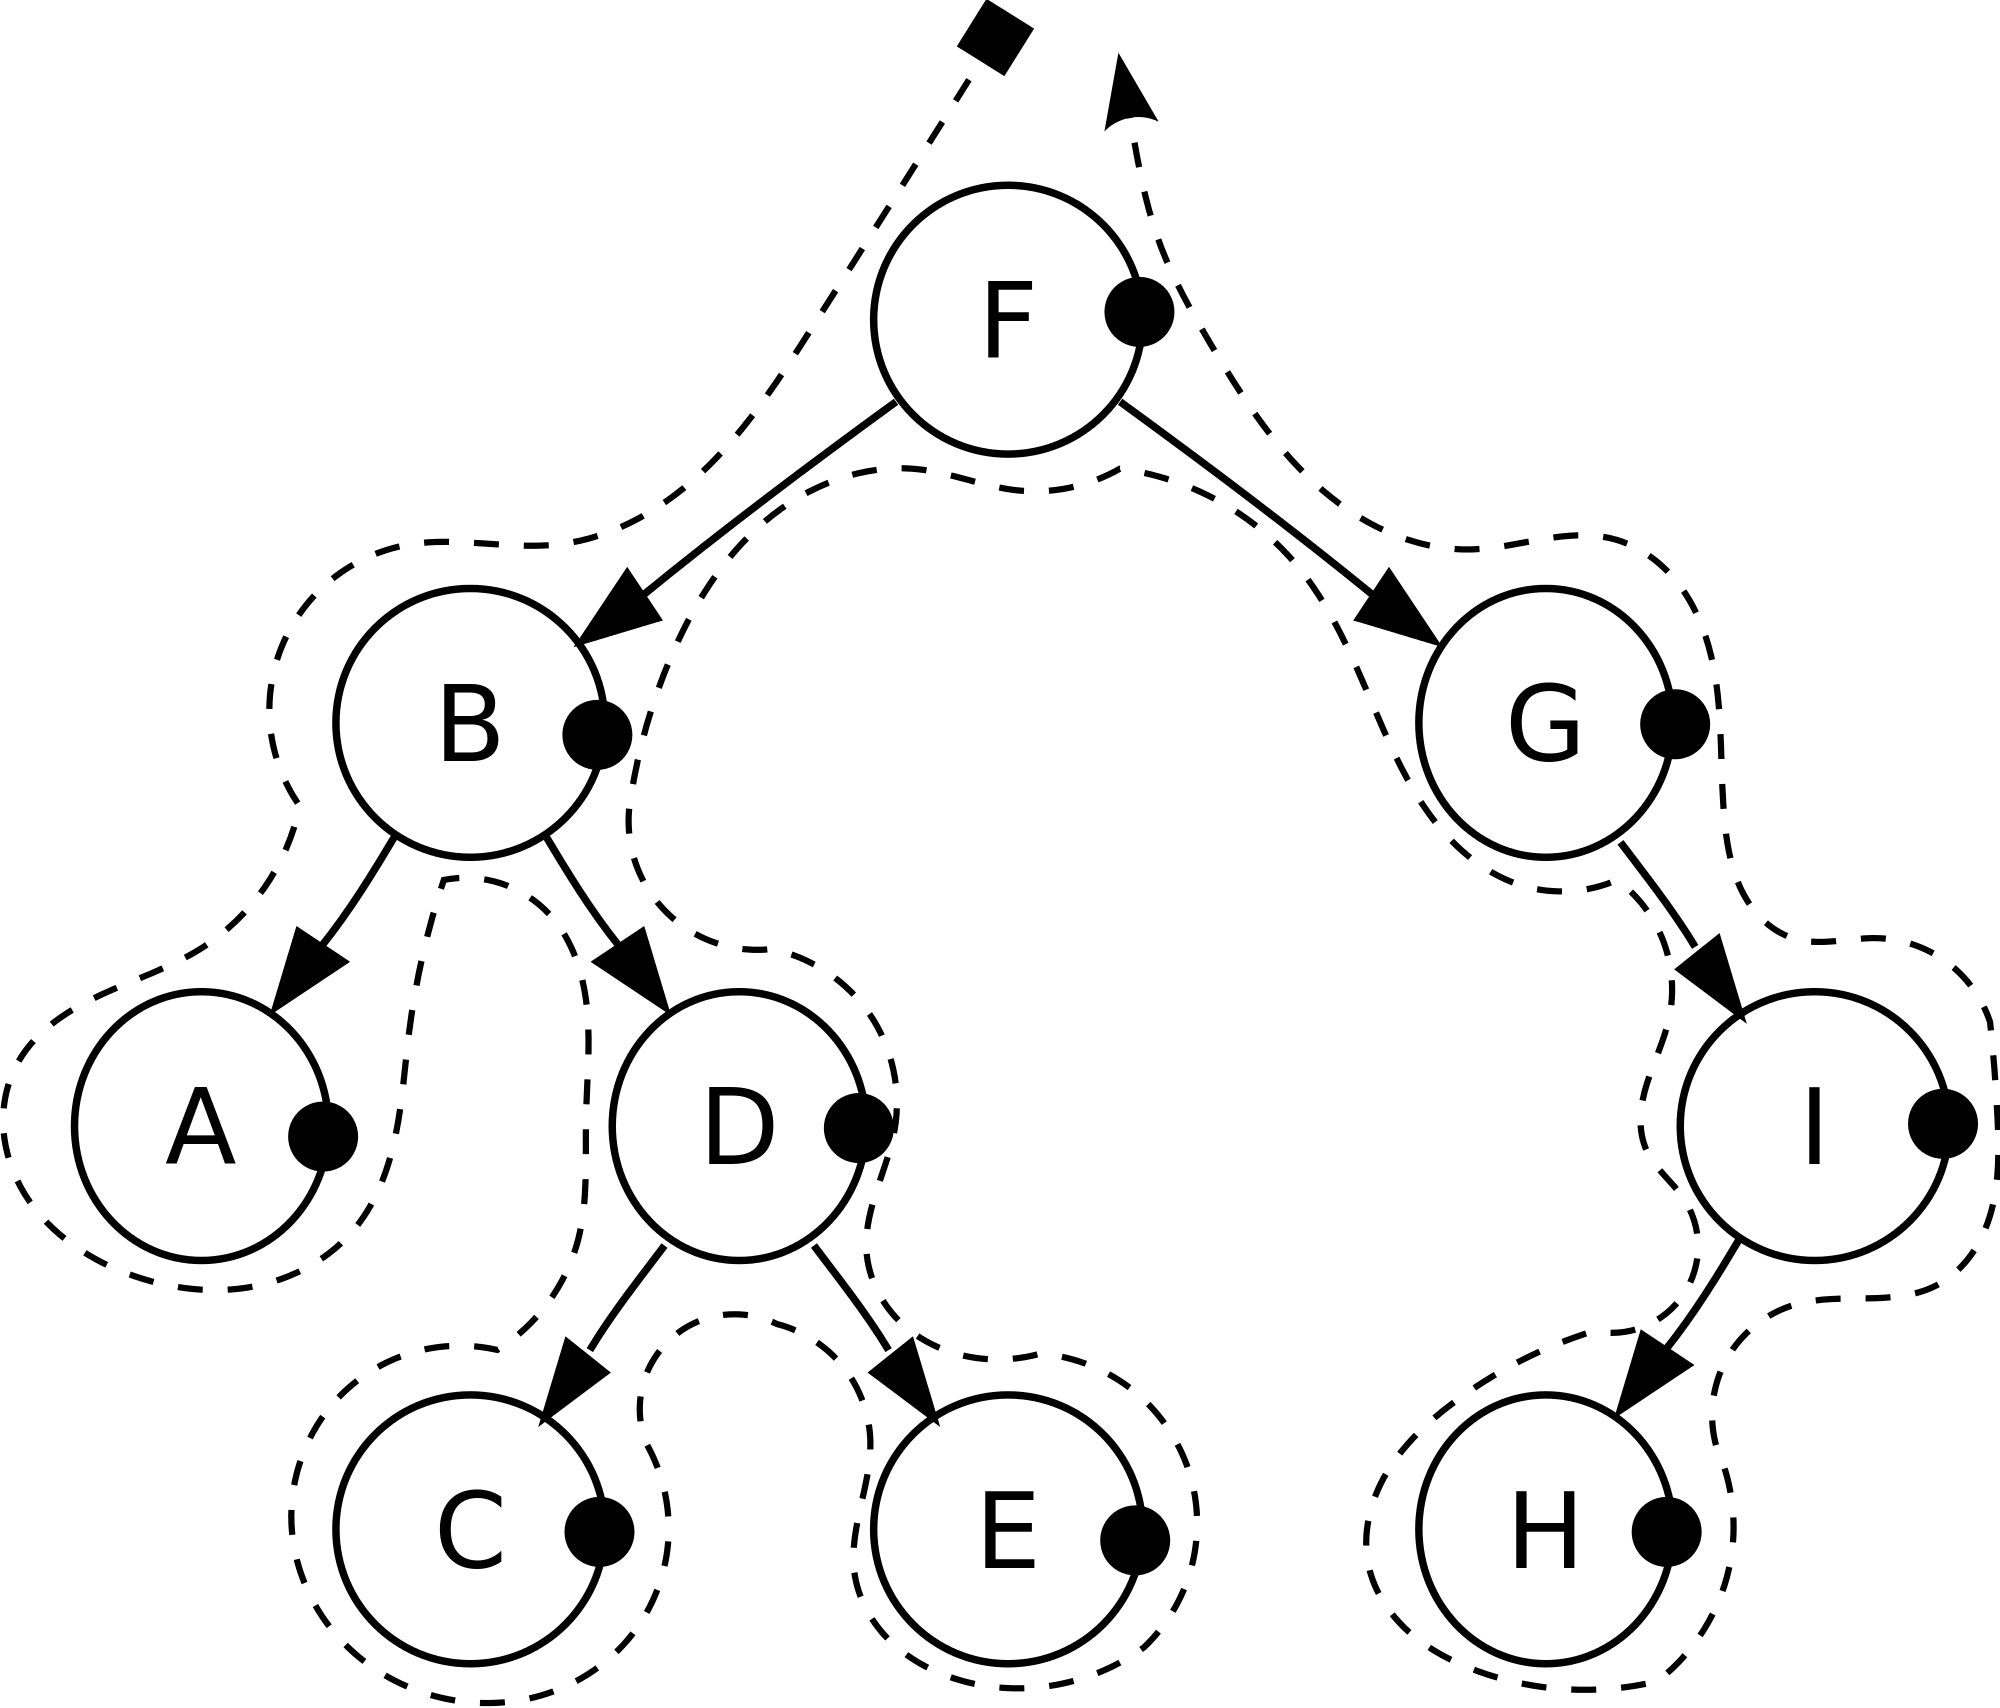
\includegraphics[width=6cm]{slides/preorder.png}
\end{center}

{\tiny image from: Wikipedia}
%(nodes arranged in memory according to a pre-order depth first traversal)
%
%\vspace{-0.1in}
%%{
%%\centering
%\begin{center}
%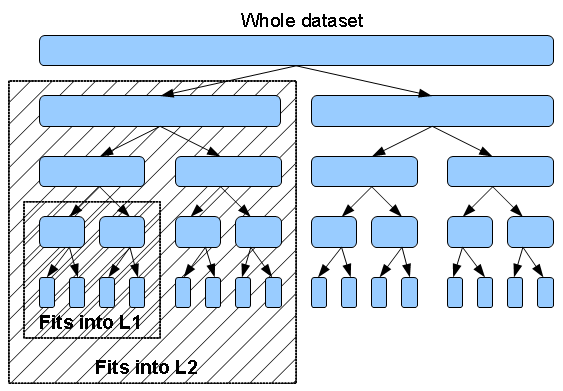
\includegraphics[width=8cm]{slides/cache_oblivious_divide}
%\end{center}
%%}
%
%\vspace{-0.1in}
%Optimal cache performance without any knowledge of the architecture
%\vspace{0.15in}

%source: 1024cores.net

\end{frame}

%%%%%%%%%%%%%%%%%%%%%%%%%%%%%%%%%%%%%%%%%%%%%%%%%%%%%%%%%%%%%%%%%%%%%%%%%%%%%%%%

\begin{frame}[fragile]{The cache efficiency of three cover tree implementations}

\centering
\graphicspath{{slides/paperimg/}}
% GNUPLOT: LaTeX picture with Postscript
\begingroup
  \makeatletter
  \providecommand\color[2][]{%
    \GenericError{(gnuplot) \space\space\space\@spaces}{%
      Package color not loaded in conjunction with
      terminal option `colourtext'%
    }{See the gnuplot documentation for explanation.%
    }{Either use 'blacktext' in gnuplot or load the package
      color.sty in LaTeX.}%
    \renewcommand\color[2][]{}%
  }%
  \providecommand\includegraphics[2][]{%
    \GenericError{(gnuplot) \space\space\space\@spaces}{%
      Package graphicx or graphics not loaded%
    }{See the gnuplot documentation for explanation.%
    }{The gnuplot epslatex terminal needs graphicx.sty or graphics.sty.}%
    \renewcommand\includegraphics[2][]{}%
  }%
  \providecommand\rotatebox[2]{#2}%
  \@ifundefined{ifGPcolor}{%
    \newif\ifGPcolor
    \GPcolortrue
  }{}%
  \@ifundefined{ifGPblacktext}{%
    \newif\ifGPblacktext
    \GPblacktextfalse
  }{}%
  % define a \g@addto@macro without @ in the name:
  \let\gplgaddtomacro\g@addto@macro
  % define empty templates for all commands taking text:
  \gdef\gplbacktext{}%
  \gdef\gplfronttext{}%
  \makeatother
  \ifGPblacktext
    % no textcolor at all
    \def\colorrgb#1{}%
    \def\colorgray#1{}%
  \else
    % gray or color?
    \ifGPcolor
      \def\colorrgb#1{\color[rgb]{#1}}%
      \def\colorgray#1{\color[gray]{#1}}%
      \expandafter\def\csname LTw\endcsname{\color{white}}%
      \expandafter\def\csname LTb\endcsname{\color{black}}%
      \expandafter\def\csname LTa\endcsname{\color{black}}%
      \expandafter\def\csname LT0\endcsname{\color[rgb]{1,0,0}}%
      \expandafter\def\csname LT1\endcsname{\color[rgb]{0,1,0}}%
      \expandafter\def\csname LT2\endcsname{\color[rgb]{0,0,1}}%
      \expandafter\def\csname LT3\endcsname{\color[rgb]{1,0,1}}%
      \expandafter\def\csname LT4\endcsname{\color[rgb]{0,1,1}}%
      \expandafter\def\csname LT5\endcsname{\color[rgb]{1,1,0}}%
      \expandafter\def\csname LT6\endcsname{\color[rgb]{0,0,0}}%
      \expandafter\def\csname LT7\endcsname{\color[rgb]{1,0.3,0}}%
      \expandafter\def\csname LT8\endcsname{\color[rgb]{0.5,0.5,0.5}}%
    \else
      % gray
      \def\colorrgb#1{\color{black}}%
      \def\colorgray#1{\color[gray]{#1}}%
      \expandafter\def\csname LTw\endcsname{\color{white}}%
      \expandafter\def\csname LTb\endcsname{\color{black}}%
      \expandafter\def\csname LTa\endcsname{\color{black}}%
      \expandafter\def\csname LT0\endcsname{\color{black}}%
      \expandafter\def\csname LT1\endcsname{\color{black}}%
      \expandafter\def\csname LT2\endcsname{\color{black}}%
      \expandafter\def\csname LT3\endcsname{\color{black}}%
      \expandafter\def\csname LT4\endcsname{\color{black}}%
      \expandafter\def\csname LT5\endcsname{\color{black}}%
      \expandafter\def\csname LT6\endcsname{\color{black}}%
      \expandafter\def\csname LT7\endcsname{\color{black}}%
      \expandafter\def\csname LT8\endcsname{\color{black}}%
    \fi
  \fi
  \setlength{\unitlength}{0.0500bp}%
  \begin{picture}(5040.00,3772.00)%
    \gplgaddtomacro\gplbacktext{%
      \csname LTb\endcsname%
      \put(1166,780){\makebox(0,0)[r]{\strut{} 0}}%
      \put(1166,1325){\makebox(0,0)[r]{\strut{} 0.2}}%
      \put(1166,1871){\makebox(0,0)[r]{\strut{} 0.4}}%
      \put(1166,2416){\makebox(0,0)[r]{\strut{} 0.6}}%
      \put(1166,2962){\makebox(0,0)[r]{\strut{} 0.8}}%
      \put(1166,3507){\makebox(0,0)[r]{\strut{} 1}}%
      \put(1661,648){\rotatebox{-45}{\makebox(0,0)[l]{\strut{}yearpredict}}}%
      \put(2023,648){\rotatebox{-45}{\makebox(0,0)[l]{\strut{}twitter}}}%
      \put(2386,648){\rotatebox{-45}{\makebox(0,0)[l]{\strut{}tinyImages}}}%
      \put(2748,648){\rotatebox{-45}{\makebox(0,0)[l]{\strut{}mnist}}}%
      \put(3111,648){\rotatebox{-45}{\makebox(0,0)[l]{\strut{}corel}}}%
      \put(3473,648){\rotatebox{-45}{\makebox(0,0)[l]{\strut{}covtype}}}%
      \put(3836,648){\rotatebox{-45}{\makebox(0,0)[l]{\strut{}artificial40}}}%
      \put(4198,648){\rotatebox{-45}{\makebox(0,0)[l]{\strut{}faces}}}%
      \put(176,2143){\rotatebox{-270}{\makebox(0,0){\strut{}cache miss rate}}}%
      \put(396,2143){\rotatebox{-270}{\makebox(0,0){\strut{}(cache misses / cache accesses)}}}%
    }%
    \gplgaddtomacro\gplfronttext{%
    }%
    \gplbacktext
    \put(0,0){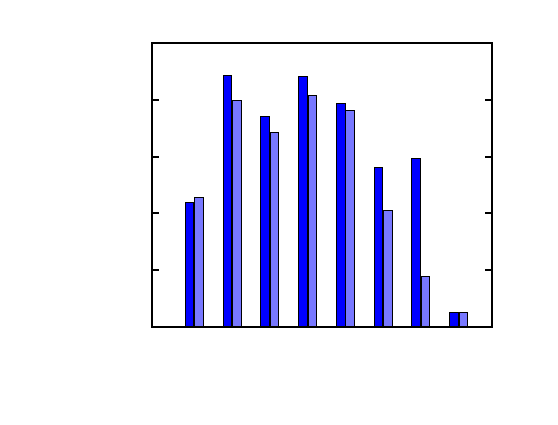
\includegraphics{cache-hlearn}}%
    \gplfronttext
  \end{picture}%
\endgroup

\definecolor{colorOrig}{RGB}{102,51,0}
\definecolor{colorMlpack}{RGB}{204,153,0}
\begin{tikzpicture}
    %\node[draw,fill=colorOrig,minimum width=0.05in,minimum height=0.3in] at (0,0) {};
    %\node at (0,0.79in) {\small\rotatebox{90}{Reference cover tree}};
    %\node[draw,fill=colorMlpack,minimum width=0.05in,minimum height=0.3in] at (0.15in,0) {};
    %\node at (0.15in,0.79in) {\small\rotatebox{90}{MLPack's cover tree}};
    %\node[draw,fill=blue,minimum width=0.05in,minimum height=0.3in] at (0.3in,0) {};
    %\node at (0.3in,0.98in) {\small\rotatebox{90}{Our cover tree (unpacked)}};
    %\node[draw,fill=lightblue,minimum width=0.05in,minimum height=0.3in] at (0.45in,0) {};
    %\node at (0.45in,0.91in) {\small\rotatebox{90}{Our cover tree (packed)}};
    \node[draw,fill=blue,minimum width=0.05in,minimum height=0.3in] at (0.3in,0) {};
    \node at (0.3in,0.98in) {\small\rotatebox{90}{Without van embde boas }};
    \node[draw,fill=lightblue,minimum width=0.05in,minimum height=0.3in] at (0.45in,0) {};
    \node at (0.45in,0.88in) {\small\rotatebox{90}{With van embde boas }};
    \node at (0,-0.475in) {};
\end{tikzpicture}

\vspace{0.15in}
Measured using Linux's \lstinline{perf stat} utility on an Amazon AWS instance
\end{frame}

%%%%%%%%%%%%%%%%%%%%%%%%%%%%%%%%%%%%%%%%%%%%%%%%%%%%%%%%%%%%%%%%%%%%%%%%%%%%%%%%
%
%\begin{frame}[fragile]{The cache efficiency of three cover tree implementations}
%
%\centering
%\graphicspath{{slides/paperimg/}}
%% GNUPLOT: LaTeX picture with Postscript
\begingroup
  \makeatletter
  \providecommand\color[2][]{%
    \GenericError{(gnuplot) \space\space\space\@spaces}{%
      Package color not loaded in conjunction with
      terminal option `colourtext'%
    }{See the gnuplot documentation for explanation.%
    }{Either use 'blacktext' in gnuplot or load the package
      color.sty in LaTeX.}%
    \renewcommand\color[2][]{}%
  }%
  \providecommand\includegraphics[2][]{%
    \GenericError{(gnuplot) \space\space\space\@spaces}{%
      Package graphicx or graphics not loaded%
    }{See the gnuplot documentation for explanation.%
    }{The gnuplot epslatex terminal needs graphicx.sty or graphics.sty.}%
    \renewcommand\includegraphics[2][]{}%
  }%
  \providecommand\rotatebox[2]{#2}%
  \@ifundefined{ifGPcolor}{%
    \newif\ifGPcolor
    \GPcolortrue
  }{}%
  \@ifundefined{ifGPblacktext}{%
    \newif\ifGPblacktext
    \GPblacktextfalse
  }{}%
  % define a \g@addto@macro without @ in the name:
  \let\gplgaddtomacro\g@addto@macro
  % define empty templates for all commands taking text:
  \gdef\gplbacktext{}%
  \gdef\gplfronttext{}%
  \makeatother
  \ifGPblacktext
    % no textcolor at all
    \def\colorrgb#1{}%
    \def\colorgray#1{}%
  \else
    % gray or color?
    \ifGPcolor
      \def\colorrgb#1{\color[rgb]{#1}}%
      \def\colorgray#1{\color[gray]{#1}}%
      \expandafter\def\csname LTw\endcsname{\color{white}}%
      \expandafter\def\csname LTb\endcsname{\color{black}}%
      \expandafter\def\csname LTa\endcsname{\color{black}}%
      \expandafter\def\csname LT0\endcsname{\color[rgb]{1,0,0}}%
      \expandafter\def\csname LT1\endcsname{\color[rgb]{0,1,0}}%
      \expandafter\def\csname LT2\endcsname{\color[rgb]{0,0,1}}%
      \expandafter\def\csname LT3\endcsname{\color[rgb]{1,0,1}}%
      \expandafter\def\csname LT4\endcsname{\color[rgb]{0,1,1}}%
      \expandafter\def\csname LT5\endcsname{\color[rgb]{1,1,0}}%
      \expandafter\def\csname LT6\endcsname{\color[rgb]{0,0,0}}%
      \expandafter\def\csname LT7\endcsname{\color[rgb]{1,0.3,0}}%
      \expandafter\def\csname LT8\endcsname{\color[rgb]{0.5,0.5,0.5}}%
    \else
      % gray
      \def\colorrgb#1{\color{black}}%
      \def\colorgray#1{\color[gray]{#1}}%
      \expandafter\def\csname LTw\endcsname{\color{white}}%
      \expandafter\def\csname LTb\endcsname{\color{black}}%
      \expandafter\def\csname LTa\endcsname{\color{black}}%
      \expandafter\def\csname LT0\endcsname{\color{black}}%
      \expandafter\def\csname LT1\endcsname{\color{black}}%
      \expandafter\def\csname LT2\endcsname{\color{black}}%
      \expandafter\def\csname LT3\endcsname{\color{black}}%
      \expandafter\def\csname LT4\endcsname{\color{black}}%
      \expandafter\def\csname LT5\endcsname{\color{black}}%
      \expandafter\def\csname LT6\endcsname{\color{black}}%
      \expandafter\def\csname LT7\endcsname{\color{black}}%
      \expandafter\def\csname LT8\endcsname{\color{black}}%
    \fi
  \fi
  \setlength{\unitlength}{0.0500bp}%
  \begin{picture}(5040.00,3772.00)%
    \gplgaddtomacro\gplbacktext{%
      \csname LTb\endcsname%
      \put(1166,780){\makebox(0,0)[r]{\strut{} 0}}%
      \put(1166,1325){\makebox(0,0)[r]{\strut{} 0.2}}%
      \put(1166,1871){\makebox(0,0)[r]{\strut{} 0.4}}%
      \put(1166,2416){\makebox(0,0)[r]{\strut{} 0.6}}%
      \put(1166,2962){\makebox(0,0)[r]{\strut{} 0.8}}%
      \put(1166,3507){\makebox(0,0)[r]{\strut{} 1}}%
      \put(1661,648){\rotatebox{-45}{\makebox(0,0)[l]{\strut{}yearpredict}}}%
      \put(2023,648){\rotatebox{-45}{\makebox(0,0)[l]{\strut{}twitter}}}%
      \put(2386,648){\rotatebox{-45}{\makebox(0,0)[l]{\strut{}tinyImages}}}%
      \put(2748,648){\rotatebox{-45}{\makebox(0,0)[l]{\strut{}mnist}}}%
      \put(3111,648){\rotatebox{-45}{\makebox(0,0)[l]{\strut{}corel}}}%
      \put(3473,648){\rotatebox{-45}{\makebox(0,0)[l]{\strut{}covtype}}}%
      \put(3836,648){\rotatebox{-45}{\makebox(0,0)[l]{\strut{}artificial40}}}%
      \put(4198,648){\rotatebox{-45}{\makebox(0,0)[l]{\strut{}faces}}}%
      \put(176,2143){\rotatebox{-270}{\makebox(0,0){\strut{}stalled CPU cycle rate}}}%
      \put(396,2143){\rotatebox{-270}{\makebox(0,0){\strut{}(stalled cycles / total cycles)}}}%
    }%
    \gplgaddtomacro\gplfronttext{%
    }%
    \gplbacktext
    \put(0,0){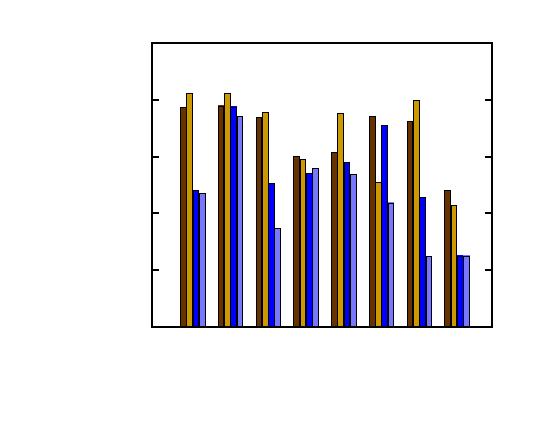
\includegraphics{stalled-front}}%
    \gplfronttext
  \end{picture}%
\endgroup

%\definecolor{colorOrig}{RGB}{102,51,0}
%\definecolor{colorMlpack}{RGB}{204,153,0}
%\begin{tikzpicture}
    %\node[draw,fill=colorOrig,minimum width=0.05in,minimum height=0.3in] at (0,0) {};
    %\node at (0,0.79in) {\small\rotatebox{90}{Reference cover tree}};
    %\node[draw,fill=colorMlpack,minimum width=0.05in,minimum height=0.3in] at (0.15in,0) {};
    %\node at (0.15in,0.79in) {\small\rotatebox{90}{MLPack's cover tree}};
    %\node[draw,fill=blue,minimum width=0.05in,minimum height=0.3in] at (0.3in,0) {};
    %\node at (0.3in,0.98in) {\small\rotatebox{90}{Our cover tree (unpacked)}};
    %\node[draw,fill=lightblue,minimum width=0.05in,minimum height=0.3in] at (0.45in,0) {};
    %\node at (0.45in,0.91in) {\small\rotatebox{90}{Our cover tree (packed)}};
    %\node at (0,-0.475in) {};
%\end{tikzpicture}
%
%\vspace{0.15in}
%Measured using Linux's \lstinline{perf stat} utility on an Amazon AWS instance
%\end{frame}

\begin{frame}[fragile]{Merging cover trees}

Merging cover trees gives us a parallel tree construction algorithm

\vspace{0.15in}

Sometimes, merging cover trees is \textbf{easy}:

\begin{center}
\begin{tikzpicture}
    [ draw
    , every node/.style={minimum size=10mm,fill=white}
    , level/.style={sibling distance = 23mm/#1, level distance=12mm}
    %,    level distance = 1.5cm}
    , sibling distance=8mm
    ]
\draw (-2.3,0) -- (8.6,0)[dotted];
\draw (-2.3,-12mm) -- (8.6,-12mm)[dotted];
\draw (-2.3,-24mm) -- (8.6,-24mm)[dotted];
\node[shape=circle,draw] at (0,0) {10}
    child { node[circle,draw] {8}
        child { node[circle,draw] {7}  }
        child { node[circle,draw] {9} }
        }
    child [color=white] {}
    %child { node[circle,draw] {12}
        %child { node[circle,draw] {9}  }
        %child { node[circle,draw] {13} }
        %}
    ;
\node[shape=circle,draw,fill=lightgreen] at (5,-12mm) {12}
    %child { node[circle,draw] {8}
        %child { node[circle,draw] {7}  }
        %child { node[circle,draw,fill=lightgreen,line width=1pt] {9} }
        %}
    %child { node[circle,draw] {12}
        child { node[circle,draw] {11}  }
        child { node[circle,draw] {13} }
        %}
    ;
\node[fill=none] at (8,3mm) {level 3};
\node[fill=none] at (8,-9mm) {level 2};
\node[fill=none] at (8,-21mm) {level 1};
\end{tikzpicture}
\end{center}

\vspace{0.1in}
No runtime bound on the merge operation, but it is fast in practice

%\vspace{0.1in}
%But, if the runtime is $o(n)$, then we get an algorithm for tree construction that takes time $O(n)$
\end{frame}

%%%%%%%%%%%%%%%%%%%%%%%%%%%%%%%%%%%%%%%%%%%%%%%%%%%%%%%%%%%%%%%%%%%%%%%%%%%%%%%%

\begin{frame}[fragile]{Merging cover trees}

Merging cover trees gives us a parallel tree construction algorithm

\vspace{0.15in}

Sometimes, merging cover trees is \textbf{hard}:

\begin{center}
\begin{tikzpicture}
    [ draw
    , every node/.style={minimum size=10mm,fill=white}
    , level/.style={sibling distance = 23mm/#1, level distance=12mm}
    %,    level distance = 1.5cm}
    , sibling distance=8mm
    ]
\draw (-2.3,0) -- (8.6,0)[dotted];
\draw (-2.3,-12mm) -- (8.6,-12mm)[dotted];
\draw (-2.3,-24mm) -- (8.6,-24mm)[dotted];
\node[shape=circle,draw] at (0,0) {10}
    child { node[circle,draw] {8}
        child { node[circle,draw] {7}  }
        child { node[circle,draw] {9} }
        }
    child [color=white] {}
    %child { node[circle,draw] {12}
        %child { node[circle,draw] {9}  }
        %child { node[circle,draw] {13} }
        %}
    ;
\node[shape=circle,draw,fill=lightred] at (5,-12mm) {11.5}
    %child { node[circle,draw] {8}
        %child { node[circle,draw] {7}  }
        %child { node[circle,draw,fill=lightgreen,line width=1pt] {9} }
        %}
    %child { node[circle,draw] {12}
        child { node[circle,draw] {11}  }
        child { node[circle,draw] {13} }
        %}
    ;
\node[fill=none] at (8,3mm) {level 3};
\node[fill=none] at (8,-9mm) {level 2};
\node[fill=none] at (8,-21mm) {level 1};
\end{tikzpicture}
\end{center}

\vspace{0.1in}
No runtime bound on the merge operation, but it is fast in practice

%\vspace{0.1in}
%But, if the runtime is $o(n)$, then we get an algorithm for tree construction that takes time $O(n)$
\end{frame}

%%%%%%%%%%%%%%%%%%%%%%%%%%%%%%%%%%%%%%%%%%%%%%%%%%%%%%%%%%%%%%%%%%%%%%%%%%%%%%%%

\begin{frame}[fragile]{The effect of parallel tree \emph{construction} on small datasets}
\begin{center}
\graphicspath{{slides/paperimg/}}
% GNUPLOT: LaTeX picture with Postscript
\begingroup
  \makeatletter
  \providecommand\color[2][]{%
    \GenericError{(gnuplot) \space\space\space\@spaces}{%
      Package color not loaded in conjunction with
      terminal option `colourtext'%
    }{See the gnuplot documentation for explanation.%
    }{Either use 'blacktext' in gnuplot or load the package
      color.sty in LaTeX.}%
    \renewcommand\color[2][]{}%
  }%
  \providecommand\includegraphics[2][]{%
    \GenericError{(gnuplot) \space\space\space\@spaces}{%
      Package graphicx or graphics not loaded%
    }{See the gnuplot documentation for explanation.%
    }{The gnuplot epslatex terminal needs graphicx.sty or graphics.sty.}%
    \renewcommand\includegraphics[2][]{}%
  }%
  \providecommand\rotatebox[2]{#2}%
  \@ifundefined{ifGPcolor}{%
    \newif\ifGPcolor
    \GPcolortrue
  }{}%
  \@ifundefined{ifGPblacktext}{%
    \newif\ifGPblacktext
    \GPblacktextfalse
  }{}%
  % define a \g@addto@macro without @ in the name:
  \let\gplgaddtomacro\g@addto@macro
  % define empty templates for all commands taking text:
  \gdef\gplbacktext{}%
  \gdef\gplfronttext{}%
  \makeatother
  \ifGPblacktext
    % no textcolor at all
    \def\colorrgb#1{}%
    \def\colorgray#1{}%
  \else
    % gray or color?
    \ifGPcolor
      \def\colorrgb#1{\color[rgb]{#1}}%
      \def\colorgray#1{\color[gray]{#1}}%
      \expandafter\def\csname LTw\endcsname{\color{white}}%
      \expandafter\def\csname LTb\endcsname{\color{black}}%
      \expandafter\def\csname LTa\endcsname{\color{black}}%
      \expandafter\def\csname LT0\endcsname{\color[rgb]{1,0,0}}%
      \expandafter\def\csname LT1\endcsname{\color[rgb]{0,1,0}}%
      \expandafter\def\csname LT2\endcsname{\color[rgb]{0,0,1}}%
      \expandafter\def\csname LT3\endcsname{\color[rgb]{1,0,1}}%
      \expandafter\def\csname LT4\endcsname{\color[rgb]{0,1,1}}%
      \expandafter\def\csname LT5\endcsname{\color[rgb]{1,1,0}}%
      \expandafter\def\csname LT6\endcsname{\color[rgb]{0,0,0}}%
      \expandafter\def\csname LT7\endcsname{\color[rgb]{1,0.3,0}}%
      \expandafter\def\csname LT8\endcsname{\color[rgb]{0.5,0.5,0.5}}%
    \else
      % gray
      \def\colorrgb#1{\color{black}}%
      \def\colorgray#1{\color[gray]{#1}}%
      \expandafter\def\csname LTw\endcsname{\color{white}}%
      \expandafter\def\csname LTb\endcsname{\color{black}}%
      \expandafter\def\csname LTa\endcsname{\color{black}}%
      \expandafter\def\csname LT0\endcsname{\color{black}}%
      \expandafter\def\csname LT1\endcsname{\color{black}}%
      \expandafter\def\csname LT2\endcsname{\color{black}}%
      \expandafter\def\csname LT3\endcsname{\color{black}}%
      \expandafter\def\csname LT4\endcsname{\color{black}}%
      \expandafter\def\csname LT5\endcsname{\color{black}}%
      \expandafter\def\csname LT6\endcsname{\color{black}}%
      \expandafter\def\csname LT7\endcsname{\color{black}}%
      \expandafter\def\csname LT8\endcsname{\color{black}}%
    \fi
  \fi
  \setlength{\unitlength}{0.0500bp}%
  \begin{picture}(5040.00,3772.00)%
    \gplgaddtomacro\gplbacktext{%
      \csname LTb\endcsname%
      \put(814,1129){\makebox(0,0)[r]{\strut{}$2^{-4}$}}%
      \csname LTb\endcsname%
      \put(814,1526){\makebox(0,0)[r]{\strut{}$2^{-3}$}}%
      \csname LTb\endcsname%
      \put(814,1922){\makebox(0,0)[r]{\strut{}$2^{-2}$}}%
      \csname LTb\endcsname%
      \put(814,2318){\makebox(0,0)[r]{\strut{}$2^{-1}$}}%
      \csname LTb\endcsname%
      \put(814,2714){\makebox(0,0)[r]{\strut{}$2^{+0}$}}%
      \csname LTb\endcsname%
      \put(814,3111){\makebox(0,0)[r]{\strut{}$2^{+1}$}}%
      \put(1539,601){\rotatebox{-45}{\makebox(0,0)[l]{\strut{}yearpredict}}}%
      \put(1539,381){\rotatebox{-45}{\makebox(0,0)[l]{\strut{}(77sec)}}}%
      \put(2242,601){\rotatebox{-45}{\makebox(0,0)[l]{\strut{}twitter}}}%
      \put(2242,381){\rotatebox{-45}{\makebox(0,0)[l]{\strut{}(107sec)}}}%
      \put(2945,601){\rotatebox{-45}{\makebox(0,0)[l]{\strut{}tinyImages}}}%
      \put(2945,381){\rotatebox{-45}{\makebox(0,0)[l]{\strut{}(65sec)}}}%
      \put(3648,601){\rotatebox{-45}{\makebox(0,0)[l]{\strut{}mnist}}}%
      \put(3648,381){\rotatebox{-45}{\makebox(0,0)[l]{\strut{}(12sec)}}}%
      \put(176,2120){\rotatebox{-270}{\makebox(0,0){\strut{}normalized tree \emph{construction} time}}}%
      \put(1464,2814){\makebox(0,0)[l]{\strut{}\tiny 1}}%
      \put(1570,2619){\makebox(0,0)[l]{\strut{}\tiny 2}}%
      \put(1667,2175){\makebox(0,0)[l]{\strut{}\tiny 4}}%
      \put(1763,1967){\makebox(0,0)[l]{\strut{}\tiny 8}}%
      \put(1860,1856){\makebox(0,0)[l]{\strut{}\tiny 16}}%
      \put(1473,3230){\makebox(0,0)[l]{\strut{}number of processors}}%
    }%
    \gplgaddtomacro\gplfronttext{%
    }%
    \gplbacktext
    \put(0,0){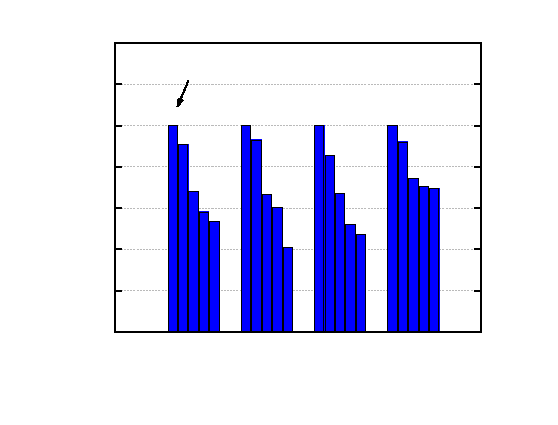
\includegraphics{parallel-ancestor-build}}%
    \gplfronttext
  \end{picture}%
\endgroup

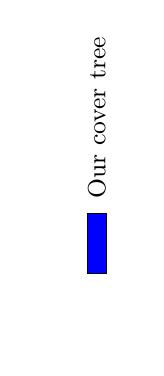
\begin{tikzpicture}
    \node[draw,fill=blue,minimum width=0.05in,minimum height=0.3in] at (0.3in,0) {};
    \node at (0.3in,0.63in) {\small\rotatebox{90}{Our cover tree}};
    \node[minimum width=0.05in,minimum height=0.3in] at (0.45in,0) {};
    \node at (0.45in,0.61in) {\small\rotatebox{90}{}};
    \node at (0,-0.475in) {};
\end{tikzpicture}
\end{center}

\vspace{0.1in}
Experiments run on an Amazon AWS instance with 16 true cores
\end{frame}

%%%%%%%%%%%%%%%%%%%%%%%%%%%%%%%%%%%%%%%%%%%%%%%%%%%%%%%%%%%%%%%%%%%%%%%%%%%%%%%%

\begin{frame}[fragile]{Parallel tree construction really matters on larger data sets}


%on small datasets with cheap metrics, parallel construction is less useful

\vspace{0.1in}
On large datasets with an expensive metric, parallelism is more useful

\vspace{0.15in}
Yahoo! Flickr dataset with 1.5 million images and earth mover distance

%\vspace{0.2in}
\vspace{0.15in}
\begin{center}
\Large
\begin{tabular}{ccccc}
\hline
num cores
 & \multicolumn{2}{c}{simplified tree} & \multicolumn{2}{c}{nearest ancestor tree} \\
%& \multicolumn{2}{c}{construction} & \multicolumn{2}{c}{construction} \\ %\cline{2-5}
& time & speedup & time & speedup \\
\hline
\hline
1  & 70.7 min & 1.0 & 210.9 min& 1.0\\
2  & 36.6 min & 1.9 & 94.2 min & 2.2\\
4  & 18.5 min & 3.8 & 48.5 min & 4.3\\
8  & 10.2 min & 6.9 & 25.3 min & 8.3\\
16 & 6.7 min & 10.5 & 12.0 min & 17.6\\
\hline
\end{tabular}
\end{center}

\end{frame}

%%%%%%%%%%%%%%%%%%%%%%%%%%%%%%%%%%%%%%%%%%%%%%%%%%%%%%%%%%%%%%%%%%%%%%%%%%%%%%%%

\begin{frame}[fragile]{The effect of parallel tree \emph{construction and query}}
\begin{center}
\graphicspath{{slides/paperimg/}}
% GNUPLOT: LaTeX picture with Postscript
\begingroup
  \makeatletter
  \providecommand\color[2][]{%
    \GenericError{(gnuplot) \space\space\space\@spaces}{%
      Package color not loaded in conjunction with
      terminal option `colourtext'%
    }{See the gnuplot documentation for explanation.%
    }{Either use 'blacktext' in gnuplot or load the package
      color.sty in LaTeX.}%
    \renewcommand\color[2][]{}%
  }%
  \providecommand\includegraphics[2][]{%
    \GenericError{(gnuplot) \space\space\space\@spaces}{%
      Package graphicx or graphics not loaded%
    }{See the gnuplot documentation for explanation.%
    }{The gnuplot epslatex terminal needs graphicx.sty or graphics.sty.}%
    \renewcommand\includegraphics[2][]{}%
  }%
  \providecommand\rotatebox[2]{#2}%
  \@ifundefined{ifGPcolor}{%
    \newif\ifGPcolor
    \GPcolortrue
  }{}%
  \@ifundefined{ifGPblacktext}{%
    \newif\ifGPblacktext
    \GPblacktextfalse
  }{}%
  % define a \g@addto@macro without @ in the name:
  \let\gplgaddtomacro\g@addto@macro
  % define empty templates for all commands taking text:
  \gdef\gplbacktext{}%
  \gdef\gplfronttext{}%
  \makeatother
  \ifGPblacktext
    % no textcolor at all
    \def\colorrgb#1{}%
    \def\colorgray#1{}%
  \else
    % gray or color?
    \ifGPcolor
      \def\colorrgb#1{\color[rgb]{#1}}%
      \def\colorgray#1{\color[gray]{#1}}%
      \expandafter\def\csname LTw\endcsname{\color{white}}%
      \expandafter\def\csname LTb\endcsname{\color{black}}%
      \expandafter\def\csname LTa\endcsname{\color{black}}%
      \expandafter\def\csname LT0\endcsname{\color[rgb]{1,0,0}}%
      \expandafter\def\csname LT1\endcsname{\color[rgb]{0,1,0}}%
      \expandafter\def\csname LT2\endcsname{\color[rgb]{0,0,1}}%
      \expandafter\def\csname LT3\endcsname{\color[rgb]{1,0,1}}%
      \expandafter\def\csname LT4\endcsname{\color[rgb]{0,1,1}}%
      \expandafter\def\csname LT5\endcsname{\color[rgb]{1,1,0}}%
      \expandafter\def\csname LT6\endcsname{\color[rgb]{0,0,0}}%
      \expandafter\def\csname LT7\endcsname{\color[rgb]{1,0.3,0}}%
      \expandafter\def\csname LT8\endcsname{\color[rgb]{0.5,0.5,0.5}}%
    \else
      % gray
      \def\colorrgb#1{\color{black}}%
      \def\colorgray#1{\color[gray]{#1}}%
      \expandafter\def\csname LTw\endcsname{\color{white}}%
      \expandafter\def\csname LTb\endcsname{\color{black}}%
      \expandafter\def\csname LTa\endcsname{\color{black}}%
      \expandafter\def\csname LT0\endcsname{\color{black}}%
      \expandafter\def\csname LT1\endcsname{\color{black}}%
      \expandafter\def\csname LT2\endcsname{\color{black}}%
      \expandafter\def\csname LT3\endcsname{\color{black}}%
      \expandafter\def\csname LT4\endcsname{\color{black}}%
      \expandafter\def\csname LT5\endcsname{\color{black}}%
      \expandafter\def\csname LT6\endcsname{\color{black}}%
      \expandafter\def\csname LT7\endcsname{\color{black}}%
      \expandafter\def\csname LT8\endcsname{\color{black}}%
    \fi
  \fi
  \setlength{\unitlength}{0.0500bp}%
  \begin{picture}(5040.00,3772.00)%
    \gplgaddtomacro\gplbacktext{%
      \csname LTb\endcsname%
      \put(1254,1129){\makebox(0,0)[r]{\strut{}$2^{-4}$}}%
      \csname LTb\endcsname%
      \put(1254,1526){\makebox(0,0)[r]{\strut{}$2^{-3}$}}%
      \csname LTb\endcsname%
      \put(1254,1922){\makebox(0,0)[r]{\strut{}$2^{-2}$}}%
      \csname LTb\endcsname%
      \put(1254,2318){\makebox(0,0)[r]{\strut{}$2^{-1}$}}%
      \csname LTb\endcsname%
      \put(1254,2714){\makebox(0,0)[r]{\strut{}$2^{+0}$}}%
      \csname LTb\endcsname%
      \put(1254,3111){\makebox(0,0)[r]{\strut{}$2^{+1}$}}%
      \put(1873,601){\rotatebox{-45}{\makebox(0,0)[l]{\strut{}yearpredict}}}%
      \put(1873,381){\rotatebox{-45}{\makebox(0,0)[l]{\strut{}(277min)}}}%
      \put(2471,601){\rotatebox{-45}{\makebox(0,0)[l]{\strut{}twitter}}}%
      \put(2471,381){\rotatebox{-45}{\makebox(0,0)[l]{\strut{}(51min)}}}%
      \put(3068,601){\rotatebox{-45}{\makebox(0,0)[l]{\strut{}tinyImages}}}%
      \put(3068,381){\rotatebox{-45}{\makebox(0,0)[l]{\strut{}(34min)}}}%
      \put(3666,601){\rotatebox{-45}{\makebox(0,0)[l]{\strut{}mnist}}}%
      \put(3666,381){\rotatebox{-45}{\makebox(0,0)[l]{\strut{}(30min)}}}%
      \put(176,2120){\rotatebox{-270}{\makebox(0,0){\strut{}normalized total runtime}}}%
      \put(396,2120){\rotatebox{-270}{\makebox(0,0){\strut{}(both \emph{construction} and \emph{query})}}}%
      \put(616,2120){\rotatebox{-270}{\makebox(0,0){\strut{}  }}}%
      \put(1774,2980){\makebox(0,0)[l]{\strut{}\tiny 1}}%
      \put(1849,3174){\makebox(0,0)[l]{\strut{}\tiny 1}}%
      \put(1924,2814){\makebox(0,0)[l]{\strut{}\tiny 1}}%
      \put(1983,2453){\makebox(0,0)[l]{\strut{}\tiny 2}}%
      \put(2058,1954){\makebox(0,0)[l]{\strut{}\tiny 4}}%
      \put(2124,1648){\makebox(0,0)[l]{\strut{}\tiny 8}}%
      \put(2184,1399){\makebox(0,0)[l]{\strut{}\tiny 16}}%
    }%
    \gplgaddtomacro\gplfronttext{%
    }%
    \gplbacktext
    \put(0,0){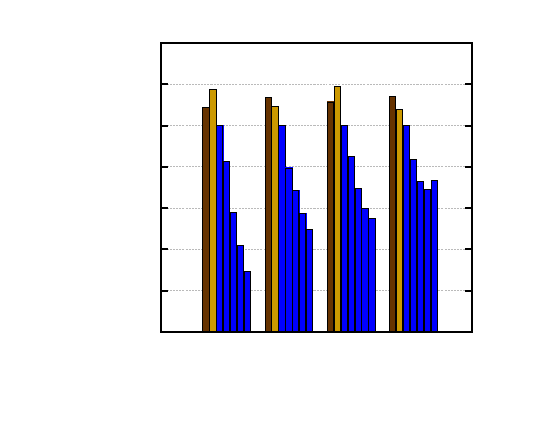
\includegraphics{parallel}}%
    \gplfronttext
  \end{picture}%
\endgroup

\definecolor{colorOrig}{RGB}{102,51,0}
\definecolor{colorMlpack}{RGB}{204,153,0}
\begin{tikzpicture}
    \node[draw,fill=colorOrig,minimum width=0.05in,minimum height=0.3in] at (0,0) {};
    \node at (0,0.79in) {\small\rotatebox{90}{Reference cover tree}};
    \node[draw,fill=colorMlpack,minimum width=0.05in,minimum height=0.3in] at (0.15in,0) {};
    \node at (0.15in,0.80in) {\small\rotatebox{90}{MLPack's cover tree}};
    \node[draw,fill=blue,minimum width=0.05in,minimum height=0.3in] at (0.3in,0) {};
    \node at (0.3in,0.63in) {\small\rotatebox{90}{Our cover tree}};
    \node[minimum width=0.05in,minimum height=0.3in] at (0.45in,0) {};
    \node at (0.45in,0.61in) {\small\rotatebox{90}{}};
    \node at (0,-0.475in) {};
\end{tikzpicture}
\end{center}

\vspace{0.1in}
Experiments run on an Amazon AWS instance with 16 true cores
\end{frame}


%%%%%%%%%%%%%%%%%%%%%%%%%%%%%%%%%%%%%%%

\begin{frame}[fragile]{Summary}

\Large

%\vspace{0.15in}
%We make cover trees even faster by:
%\begin{itemize}
%\item Providing a simpler definition of the cover tree that reduces the number of nodes from $O(n)$ to exactly $n$
%\item Introducing the ``nearest ancestor'' invariant
%\item Improving cache performance
%\item Constructing the tree in parallel
%\end{itemize}

You should use cover trees.

\vspace{0.35in}
We made them easier to implement and faster.

\vspace{0.35in}
%\rule{\textwidth}{1pt}
%\vspace{-0.10in}

All the code is licensed under the BSD3 and available at:

\begin{center}
\url{http://github.com/mikeizbicki/hlearn}
\end{center}

%It's written in Haskell.

\end{frame}



%%%%%%%%%%%%%%%%%%%%%%%%%%%%%%%%%%%%%%%%%%%%%%%%%%%%%%%%%%%%%%%%%%%%%%%%%%%%%%%%


\end{document}



